For \(a_1\), there are only 3 possible distinct non-empty coverings: 1 triangle, 2 triangles, and 3 triangles. 

\begin{enumerate}
    \item For 1 triangle, the diameter of the set is \(\frac{1}{2}\), the proportion covered is \(\frac{1}{3}\), so the value of \(a_1\) is \(\frac{(1/2)^s}{(1/3)} = 1\);
    \item For 2 triangles, the diameter is 1, while the proportion covered is \(\frac{2}{3}\), notably less than 1: thus this will result in a higher value for \(a_1\);
    \item For 3 triangles, the diameter is 1, the proportion covered is 1, hence our value is also 1.
\end{enumerate}

Hence \(a_1 = 1\).

For \(a_2\), we need to do a similar job -- but we can ignore coverings which have points in only one of the 3 largest triangles due to these being equivalent to colourings of \(a_1\). This is clear as if we have a covering of \(T_n\), we can scale it down by scale factor \(\frac{1}{2}\) centred at \((0,0)\) to cover one of the three largest triangles of \(T_{n+1}\). This is clearly a covering as these triangles have been scaled down in a similar fashion to the first contraction function in the IFS, thus it's the same as just adding this function to the beginning of \(S_{I_n}(\Delta)\). This will have half the diameter, and have \(\frac{1}{3}\) of the measure (as there are 3 identical largest triangles that could be filled). Thus letting \(D\) be the diameter, and \(M\) be the measure, our value for \(a_{i+1}\) is \(\frac{(D/2)^s}{M/3} = \frac{D^s}{M}\), which is the same value as our covering for \(a_i\). Thus our lemma is proven. 

Therefore, there are then 2 cases to consider: if one of the corner triangles is filled, and if one of the corner triangles is not filled. 

I claim the best answer is when we pick the 6 triangles closest to the centre empty triangle: this would give an answer of
\[\frac{0.75^{\log(2)/\log(3)}}{\frac{6}{9}} = \frac{3^{\log(3)/\log(2) - 1}}{2} = 0.95075.\]

If one of the corner triangles is filled, we may as well fill out the 3 triangles in the sub-triangle of that corner triangle (as we must have one outside this sub-triangle anyway.) If we use a triangle adjacent to this sub-triangle, we may as well also have the one symmetrically opposite (as this doesn't increase the diameter) But this only covers 5 triangles with the same diameter as last time so can't be better.

If we choose one of the other corner triangles, we may as well cover the whole triangle anyway but this would just give us a value of 1. If we don't choose the corner triangles but use all the other triangles, this gives us a diameter of \(\frac{\sqrt{13}}{4}\), and a measure of \(\frac{7}{9}\): plugging this into the formula we get a value of around 1.09 which is worse than the trivial bound of 1.

The other case is if we don't pick any of the corners. Then there are really only two cases to consider: picking 3 adjacent triangles and picking all 6 triangles. If we pick 3 adjacent triangles, this gives us a diameter of greater than \(\frac{1}{2}\) but the same number of triangles as if we just picked one of the sub-triangles with 3 triangles - thus it's strictly worse than that bound. The other case is the best bound shown earlier - hence we are done and
\[a_2 = \frac{3^{\log(3)/\log(2) - 1}}{2}.\]

The diagram below shows the choice of triagnles for \(a_2\).

\begin{center}
    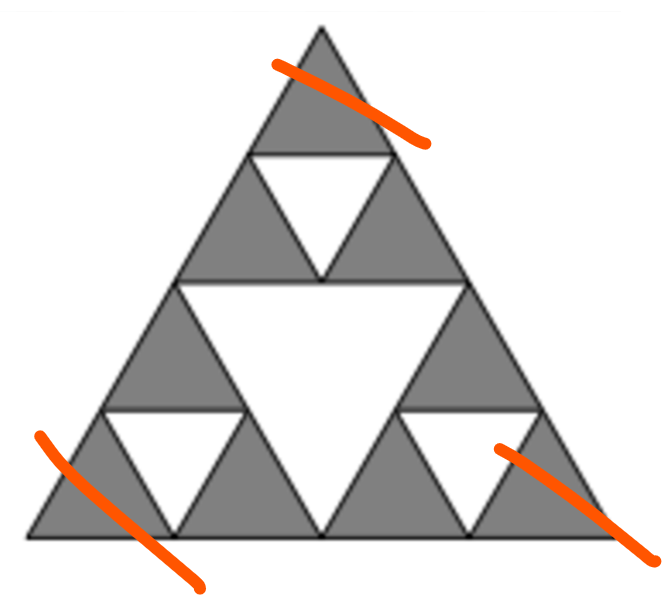
\includegraphics[width=0.5\linewidth]{solutions/section-5-0/diag-5-0-2.png}
\end{center}